\label{sec:chunk_generation}
\begin{figure*}
  %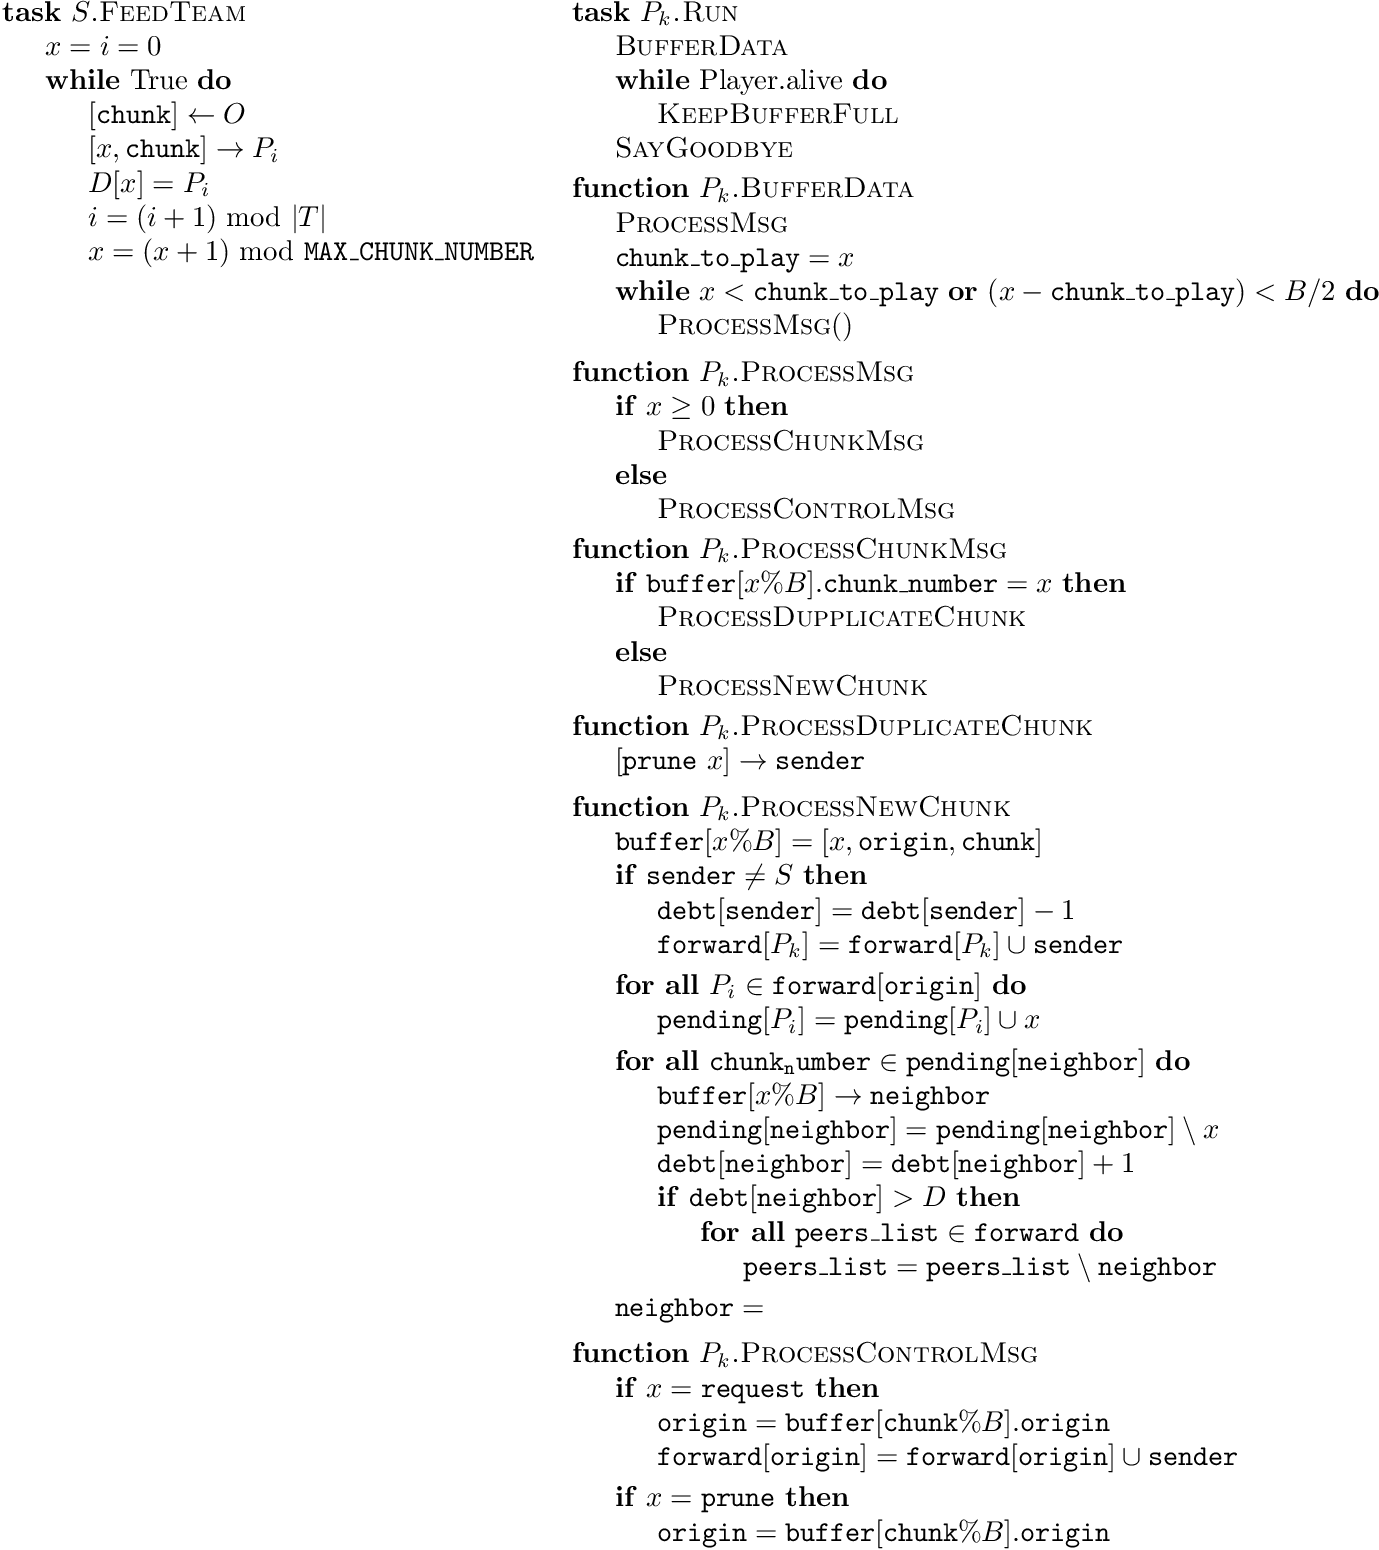
\includegraphics[width=0.75\textwidth]{chunk_generation_and_flooding}
  \fig{170}{3cm}{splitter_chunk_generation}
  \caption{Chunk generation at the splitter.\label{fig:chunk_generation}}
\end{figure*}
The splitter $S$ divides the stream into chunks of data
($\mathtt{chunk}$) of constant length $C$, and sends exclusively each
chunk to a different \emph{origin peer} $P_i\in T$, using a
round-robin schema (see Fig.~\ref{fig:chunk_generation}). Each chunk
is enumerated with an index $x$, conforming a message
$[c_x]=[x,\mathtt{chunk}]$, where $x=i~\mathrm{mod}~|T|$.

We define a \emph{round} (in a team) as the time necessary to send two
consecutive chunks from the splitter (of such team) to the same peer,
using the round-robing. This time is variable and depends on $|T|$,
$C$, and the average bit-rate of the media, $A$.

\begin{comment}
The round-time is defined by:
\begin{equation}
  \cal{r} = \cal{c}N.
  \label{eq:round_time}
\end{equation}
For example, if we use only one team of $N=256$ peers, a chunk size
$C=1024$~bytes, and a video of $1$~Mb/s, the round time is
\begin{displaymath}
  \cal{r} = \frac{1024\frac{\text{bytes}}{\text{chunk}}\times
    8\frac{\text{bits}}{\text{byte}}}{10^6\frac{\text{bits}}{\text{second}}}\times
  256 \approx 2.1~\text{seconds}.
\end{displaymath}
\end{comment}
